\section{Control}
So far we have analyzed our system as a continuous system.
However, we are using the Raspberry Pi to control the robot, so we will
be using digital control. It's a branch of control theory that uses
digital computers to act as system controllers.

In order to sample the position and the speed we use the rotatory encoders.
They count the number of flags so there is a constant to convert them in to radiants.

All our digital control was made in periodical loops. To get the speed we
divided the incremental position by the period of the loop. All the controllers
are PID controllers each of time with different inputs, constants and outputs.

A PID controller continuously calculates an error value $e(t)$ as the difference between
a desired set point and a measured process variable and applies a
correction based on proportional, integral, and derivative terms
(denoted P, I, and D respectively).

To adjust the controller constants in all cases we did the following way:

\begin{enumerate}
    \item Set all gains to zero.
    \item Increase the $P$ gain until the response to a disturbance is steady oscillation.
    \item Increase the $D$ gain until the oscillations go away (i.e. it's critically damped).
    \item Repeat steps 2 and 3 until increasing the D gain does not stop the oscillations.
    \item Set P and D to the last stable values.
    \item Increase the $I$ gain until it brings you to the set point with no oscillations desired.
\end{enumerate}

\subsection{Position control}
The first steep was to control the position of a peg attached to the motor.
We started by making sure that the encoder was reading the correct position.


\begin{figure}[H]
    \centering
    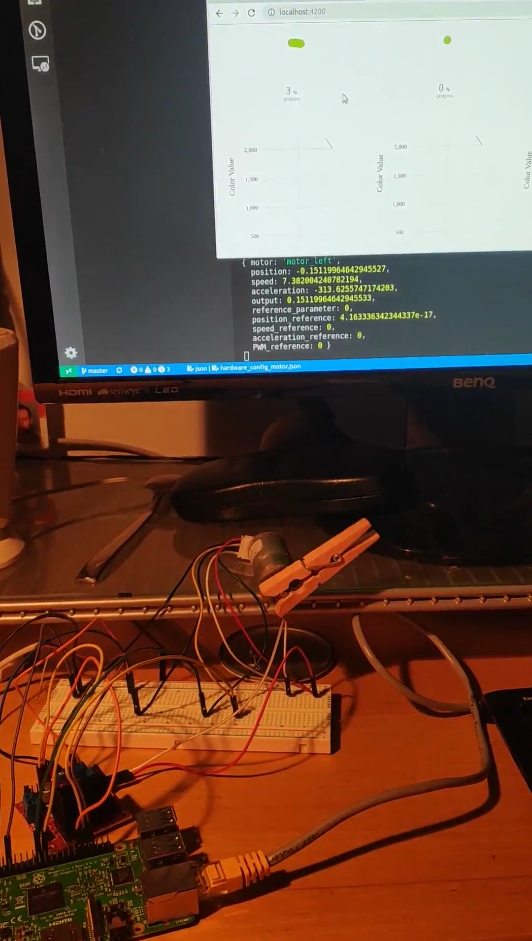
\includegraphics[width=7cm]{img/peg.png}
    \caption{Picture of the set up to control the peg.}
    \label{fig: MPU-6050}
\end{figure}


\subsection{Speed control}

\subsection{Inclination control}